\documentclass[10pt]{beamer}

\usetheme{AnnArbor}
\usepackage{appendixnumberbeamer}
\usepackage{tikz}

\usepackage{booktabs}
\usepackage[scale=2]{ccicons}

\usepackage{xspace}
\newcommand{\themename}{\textbf{\textsc{metropolis}}\xspace}

\usepackage[
backend=biber,
style=numeric,
]{biblatex}
\addbibresource{bibliography.bib}

\usepackage{xcolor}
\usepackage{listings}

\lstdefinestyle{mypython}{
  language=Python,
  basicstyle=\ttfamily\small,
  keywordstyle=\color{blue}\bfseries,
  stringstyle=\color{red},
  commentstyle=\color{gray},
  showstringspaces=false,
  breaklines=true,
  columns=fullflexible,
}

\lstset{style=mypython}

% \bibliography{gpr}

\title[Simulation Framework]{Simulation Framework}
\subtitle{First Approach at a Python-first General Simulation Package}
\date{\today}
\author{Matt McAnear}
\institute[UofM]{Dept. of Statistics, University of Michigan}


% \titlegraphic{\hfill\includegraphics[height=1.5cm]{logo.pdf}}

\begin{document}

\maketitle

\AtBeginSection[]{
  \begin{frame}
  \vfill
  \centering
  \begin{beamercolorbox}[sep=8pt,center,shadow=true,rounded=true]{title}
    \usebeamerfont{title}\insertsectionhead\par%
  \end{beamercolorbox}
  \vfill
  \end{frame}
}

\setbeamertemplate{caption}[numbered]
\setbeamertemplate{section in toc}[sections numbered]

\subsection[Introduction]{Introduction}

\begin{frame}{Current Simulation Frameworks}

Major simulation frameworks are currently all in R.

\begin{itemize}
  \item simR \cite{green_simr_2016}\cite{sigal_play_2016}
  \item simchef \cite{duncan_simchef_2024}
  \item simulator \cite{bien_simulator_2016}
\end{itemize}

This is basically absent from Python.

\end{frame}


\begin{frame}
  
  \frametitle{Values}

  \begin{itemize}
    \item It should feel like Python
    \item Composition over Inheritance
    \item Functional Style
    \item Modular
    \item Natural Vectorization
  \end{itemize}
  
\end{frame}

\section{Design}

\begin{frame}
  \frametitle{Core Components}

  \begin{itemize}
    \item \textbf{Models}: Data Generating Processes
    \item \textbf{Methods}: Procedures to be applied to data
    \item \textbf{Metrics}: Performance Measures
    \item \textbf{Visualizations}: Orchestration of the above
  \end{itemize}
\end{frame}

\begin{frame}{Architecture}

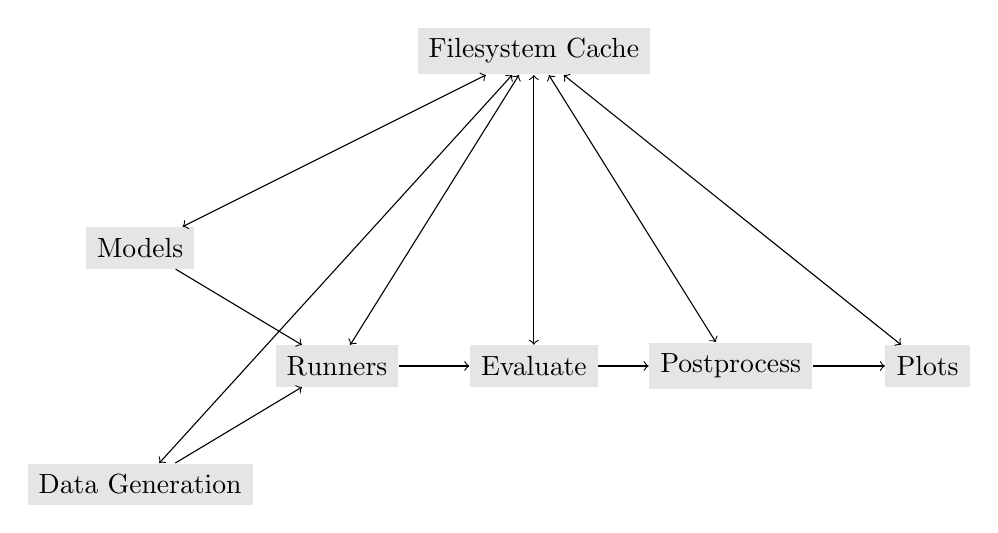
\begin{tikzpicture}
\tikzstyle{component}=[rectangle,fill=black!10,minimum size=12pt,inner sep=4pt]


\node[component](Models) at (0,7.5){Models};
\node[component](Data) at (0,4.5){Data Generation};
\node[component](Runners) at (2.5,6){Runners};
\node[component](Evaluate) at (5,6){Evaluate};
\node[component](Filesystem) at (5,10){Filesystem Cache};
\node[component](Postprocess) at (7.5,6){Postprocess};
\node[component](Plots) at (10,6){Plots};
\draw[->] (Data) -- (Runners);
\draw[<->] (Data) -- (Filesystem);
\draw[->] (Models) -- (Runners);
\draw[<->] (Models) -- (Filesystem);
\draw[->] (Runners) -- (Evaluate);
\draw[<->] (Runners) -- (Filesystem);
\draw[->] (Evaluate) -- (Postprocess);
\draw[<->] (Evaluate) -- (Filesystem);
\draw[<->] (Postprocess) -- (Filesystem);
\draw[->] (Postprocess) -- (Plots);
\draw[<->] (Plots) -- (Filesystem);

\end{tikzpicture}

\end{frame}

\begin{frame}{Component Details}
  \begin{itemize}
    \item Data Generation
      \begin{itemize}
        \item Tag arbitrary functions as data generators
        \item Returns data sets as tensor-like structures for easier vectorization
        \item Automatically create an output type
      \end{itemize}
    \item Models
      \begin{itemize}
        \item Align inputs with output of data generators
        \item Tag method outputs and create output types
        \item Run model fitting with a given set of model fitting hyperparameters
      \end{itemize}
        \item Runners
          \begin{itemize}
            \item Orchestrate / match data generators and models
            \item Run only if results are not present
            \item Align randomization
            \item Control Caching
          \end{itemize}
      \end{itemize}
\end{frame}

\begin{frame}{Component Details}
  \framesubtitle{(continued)}
  \begin{itemize}
    \item Evaluate
    \begin{itemize}
      \item Provide Standard Metrics
      \item Tag arbitrary functions as metrics
      \item Align inputs with model outputs
    \end{itemize}
    \item Postprocess
      \begin{itemize}
        \item Aggregate results or fit models on results
        \item Allow for arbitrary functions of outputs that aren't strictly evaluation
      \end{itemize}
    \item Plot
  \end{itemize}

\end{frame}

\section{Demonstration}

\begin{frame}[fragile]{Simple DGP}
  
\begin{lstlisting}
## Usage
@data_generator("Linear Data", output=("X", "y", "beta"))
def ols_data(N, p):
    X = rng.normal(size=(N, p))
    beta = rng.normal(size=p)
    y = X @ beta + rng.normal(size=N)
    return X, y, beta
    
## Output
output_tuple = ols_data(N=100, p=10)
assert output_tuple.X.shape == (100, 10)
assert output_tuple.y.shape == (100,)
assert output_tuple.beta.shape == (10,)
\end{lstlisting}
  
\end{frame}

\begin{frame}[fragile]{Simple Method}
  
\begin{lstlisting}
## Usage
@model("Ridge", output="beta")
def ridge_model(X, y, lam=1.0):
    p = X.shape[1]
    eye = np.eye(p)

    beta = np.linalg.solve(X.T @ X + lam * eye, X.T @ y)
    return beta
\end{lstlisting}
  
\end{frame}


\begin{frame}[fragile]{Running A Simulation}

\begin{lstlisting}
# The Happy Path
Runner = SimRunner(
    data_generator=ols_data,
    method=ridge_model,
    sim_params={
        "Linear Data": {"N": [50, 100], "p": [5, 10, 20]},
        "Ridge": {"lam": [0.1, 0.5, 1.0, 1.5]},
    },
)

results = Runner.run_simulations(N_sims)
\end{lstlisting}
\end{frame}


\begin{frame}[fragile]{Running a Simulation}
  \framesubtitle{(continued)}
  \begin{lstlisting}
# Inside the runner class; the idea is to match the output
# arguments from a class with the input values from the method
# signature using the `inspect` library
def _run_scenario(self, scenario, N_sims):
  dgp_args, method_args = self._parse_scenario_args(scenario)

  for _ in range(N_sims):
    sim_data = self.data_generator(**dgp_args)

    shared_params = set(sim_data._fields).intersection(
        inspect.signature(self.method.fn).parameters
    )

    method_inputs = {k: sim_data.__getattribute__(k) for k in shared_params}

    method_output = self.method(**method_inputs, **method_args)

    return method_output
  \end{lstlisting}
\end{frame}

\section{Conclusion}

\begin{frame}{Lots left to do}

  \begin{itemize}
    \item Play with the R versions to get a better feel for features
    \item Add filesystem based caching
    \item Simplify the handoff of function outputs to next stage in simulation pipeline
    \item Solidify random number generation / state
  \end{itemize}
\end{frame}

\begin{frame}[allowframebreaks]{Works Cited}
  \printbibliography
\end{frame}

\end{document}
